\section{Pregunta 1 (0.2 puntos)}
\def\checkmark{\tikz\fill[scale=0.4](0,.35) -- (.25,0) -- (1,.7) -- (.25,.15) -- cycle;}


¿Cuáles son los criterios de parada del algoritmo del método de newton con entradas ($f(x)$, $x_{0}$, tolerancia, número de iteraciones)?:

\begin{itemize}
    \item $f(x) < 0$
    \item $|x_{n} - x_{n-1}| < tolerancia$ \checkmark
    \item $\frac{df(x)}{dx} < 0$
    \item $n >$ número $de iteraciones$ \checkmark
\end{itemize}

\section{Pregunta 2 (0.2 puntos)}

Si se busca encontrar la raíz $x_{v}$ para la función $f(x)=h(x)(x-X_{v})^2$
donde $h(x)$ representa cualquier función continua y diferenciable, no es
aconsejable usar el método de Newton modificado (Newton II raíces múltiples).
PORQUE las primeras 2 derivadas de la función $f(x)=h(x)(x-X_{v})^2$ son iguales
a cero en $x_{v}$ y esto causa que existan divisiones por cero en el método de
Newton modificado (Newton II raices múltiples).

\begin{itemize}
    \item La afirmación y razón son verdaderas y la razón explica correctamente la afirmación.
    \item La afirmación y razón son verdaderas pero la razón NO explica correctamente la afirmación.
    \item La afirmación es verdadera pero la  razón es falsa. \checkmark
    \item La afirmación es falsa pero la  razón es verdadera.
    \item La afirmación y razón son falsas.
\end{itemize}

\section{Pregunta 3 (0.2 puntos)}

La norma 3 para el vector $v = [v_{1} v_{2} v_{3}]$ es:

\begin{itemize}
    \item $(v_{1} + v_{2} + v_{3})^3$
    \item $\sqrt[3]{|v_{1}|^3 + |v_{2}|^3 + |v_{3}|^3}$ \checkmark
    \item $|v_{1}|^3 + |v_{2}|^3 + |v_{3}|^3$
    \item $v_{1}^3 + v_{2}^3 + v_{3}^3$
    \item $\sqrt[3]{v_{1}^3 + v_{2}^3 + v_{3}^3}$
\end{itemize}

\section{Pregunta 4 (0.2 puntos)}

 (Análisis de Relación) La matriz,
\[ A =
    \begin{bmatrix}
        15 & 2  & 3  \\
        0  & -6 & -6 \\
        0  & 0  & -4
    \end{bmatrix}
\]

es triangular inferior PORQUE en toda matriz triangular inferior los coeficientes
$a_{ij} = 0$ para todo $j > i$.

\begin{itemize}
    \item La afirmación y la razón son VERDADERAS y la razón es una explicación CORRECTA
          de la afirmación.
    \item La afirmación y la razón son VERDADERAS, pero la razón NO es una explicación CORRECTA
          de la afirmación.
    \item La afirmación es VERDADERA, pero la razón es una proposición FALSA.
    \item La afirmación es FALSA, pero la razón es una proposición VERDADERA. \checkmark
    \item La afirmación como la razón son proposiciones FALSAS.
\end{itemize}

\section{Pregunta 5 (0.2 puntos)}

Cuando se busca resolver un sistema de ecuaciones con la factorización LU, podemos afirmar que:

\begin{itemize}
    \item Se debe usar el método de eliminación Gaussiana con pivoteo total para calcular  la factorización LU.
    \item Se debe calcular un proceso de sustitución regresiva y de sustitución progresiva. \checkmark
    \item L es una matriz triangular inferior y U una matriz triangular superior \checkmark
    \item Se aumenta la cantidad de operaciones en sistemas con vector de entradas variable.
\end{itemize}

\section{Pregunta 6, VAMOSSSS MESSI!!! (0.2 puntos)}

\begin{figure}[H]
    \centering
    \begin{subfigure}[b]{0.5\textwidth}
        \centering
        
\includegraphics[width=0.5\textwidth]{Figures/0. General/ALIEN.jpg}
        \caption{Alien stuff}
        \label{fig: Nasca Alien}
    \end{subfigure}
\end{figure}

Con el descubrimiento de las momias de Nazca en la cámara de diputados de
México, los diferentes extraterrestres que habitan la Tierra se reunieron para
discutir dónde van a vivir, ya que la mayoría se mantenía en las sombras pero
ahora pueden salir fácilmente sin que los molesten los hombres de negro. Alf
propone que deben vivir en Estados Unidos y cumplir el sueño Americano, por
otro lado Thor propone vivir en Noruega para más friito, Clark Kent dice que es
mejor un pueblito tipo Smallville, mientras que Gokú propone una isla cerca de
Japón. Al final, ET, que es el que tiene más experiencia en eso de buscar
"Hogar", dice que deben vivir en Medellín ya que allí aceptan muy bien a los
extranjeros y nómadas digitales, el único problema es que el arriendo que deben
pagar allí se sube mucho a medida que lleguen más extraterrestres.
La función que relaciona la cantidad de extraterrestres $E$ con el precio del
arriendo $x$ en doláres, es:

\[E = \pi^{-x}(-1 + x) + x^{\frac{2}{3}}\]

\subsection{1.5 pts}

Ayude a Alf y los "muchachos" a saber en cuánto les sale el arriendo en Metrallo
si la cantidad de extraterrestres que llegan son los últimos dos dígitos de su
cédula (En este caso el número 10). Use el método de Newton
con 6 cifras significativas y con condiciones iniciales $X_{0} = C$ donde $C$
es los últimos dos dígitos de su cédula (En este caso el número 10).
Entregue la tabla solución con el número de iteraciones, $X_{n}$, $f(X_{n})$ y Error.

Dado que la cantidad de extraterrestres \( E \) y el precio del arriendo \( x \) están relacionados por la ecuación
\[ E = \pi^{-x}(-1 + x) + x^{\frac{2}{3}} \]
queremos encontrar \( x \) cuando \( E = 10 \). Esto se traduce en resolver la ecuación:
\[ 10 = \pi^{-x}(-1 + x) + x^{\frac{2}{3}} \]

Para el método de Newton necesitamos la derivada de la función
\[ f(x) = \pi^{-x}(-1 + x) + x^{\frac{2}{3}} - 10 \]
La derivada \( f'(x) \) es:
\[ f'(x) = \frac{ln(\pi) \pi^{-x} (-1+x)}{\pi^x} + \frac{2x^{-\frac{1}{3}}}{3} \]

La fórmula de iteración del método de Newton es:
\[ X_{n+1} = X_n - \frac{f(X_n)}{f'(X_n)} \]

\begin{tabular}{|c|c|c|c|}
    \hline
    \textbf{Iteración} & \( X_{n} \)        & \( f(X_{n}) \)          & \textbf{Error}         \\
    \hline
    1                  & 27.316209708393743 & -0.929867625373193      & 17.316209708393743     \\
    \hline
    2                  & 31.516885840772787 & -0.022336209813614616   & 4.200676132379044      \\
    \hline
    3                  & 31.62271739457353  & -1.2481958698629114e-05 & 0.10583155380074416    \\
    \hline
    4                  & 31.6227766016653   & -3.893774191965349e-12  & 5.920709176976402e-05  \\
    \hline
    5                  & 31.62277660168377  & 0.0                     & 1.8470558416083804e-11 \\
    \hline
\end{tabular}

\subsection{1.5 pts}

Roger que es un Alien más bien pirobo, les asegura que el método usado no es
bueno, porque la $g(x)$ de este método no es buena función de punto fijo; pero
Messi por el contrario dice que sí es buena. Determine gráficamente si la
función $g(x)$ del método de Newton es buena función de punto fijo en el
intervalo [$X_{s} - C$, $X_{s} + C$], donde $X_{s}$ es la solución del ejercicio
anterior. Entregue su procedimiento gráfico, y determine cuál Alien tiene razón.

Para determinar si \( g(x) \) es una buena función de punto fijo, es necesario verificar que en el intervalo de interés, la derivada de \( g(x) \) está entre -1 y 1, es decir, \( |g'(x)| < 1 \).

Dado que:
\[ X_s \approx 31.6228 \]
\[ C = 10 \]

Podemos calcular el intervalo \([X_s - C, X_s + C]\):

\begin{enumerate}
    \item \textbf{Límite inferior del intervalo}:
          \[ X_s - C = 31.6228 - 10 = 21.6228 \]
    \item \textbf{Límite superior del intervalo}:
          \[ X_s + C = 31.6228 + 10 = 41.6228 \]
\end{enumerate}

Por lo tanto, el intervalo es \([21.6228, 41.6228]\).

Dentro de este intervalo, es necesario evaluar \( g'(x) \) para asegurar que \( |g'(x)| < 1 \). Si este criterio se satisface en todo el intervalo, entonces \( g(x) \) es una buena función de punto fijo y Messi tiene razón. Si no se cumple este criterio en algún punto del intervalo, entonces Roger tiene razón.

\begin{figure}[H]
    \centering
    \begin{subfigure}[b]{\textwidth}
        \centering
        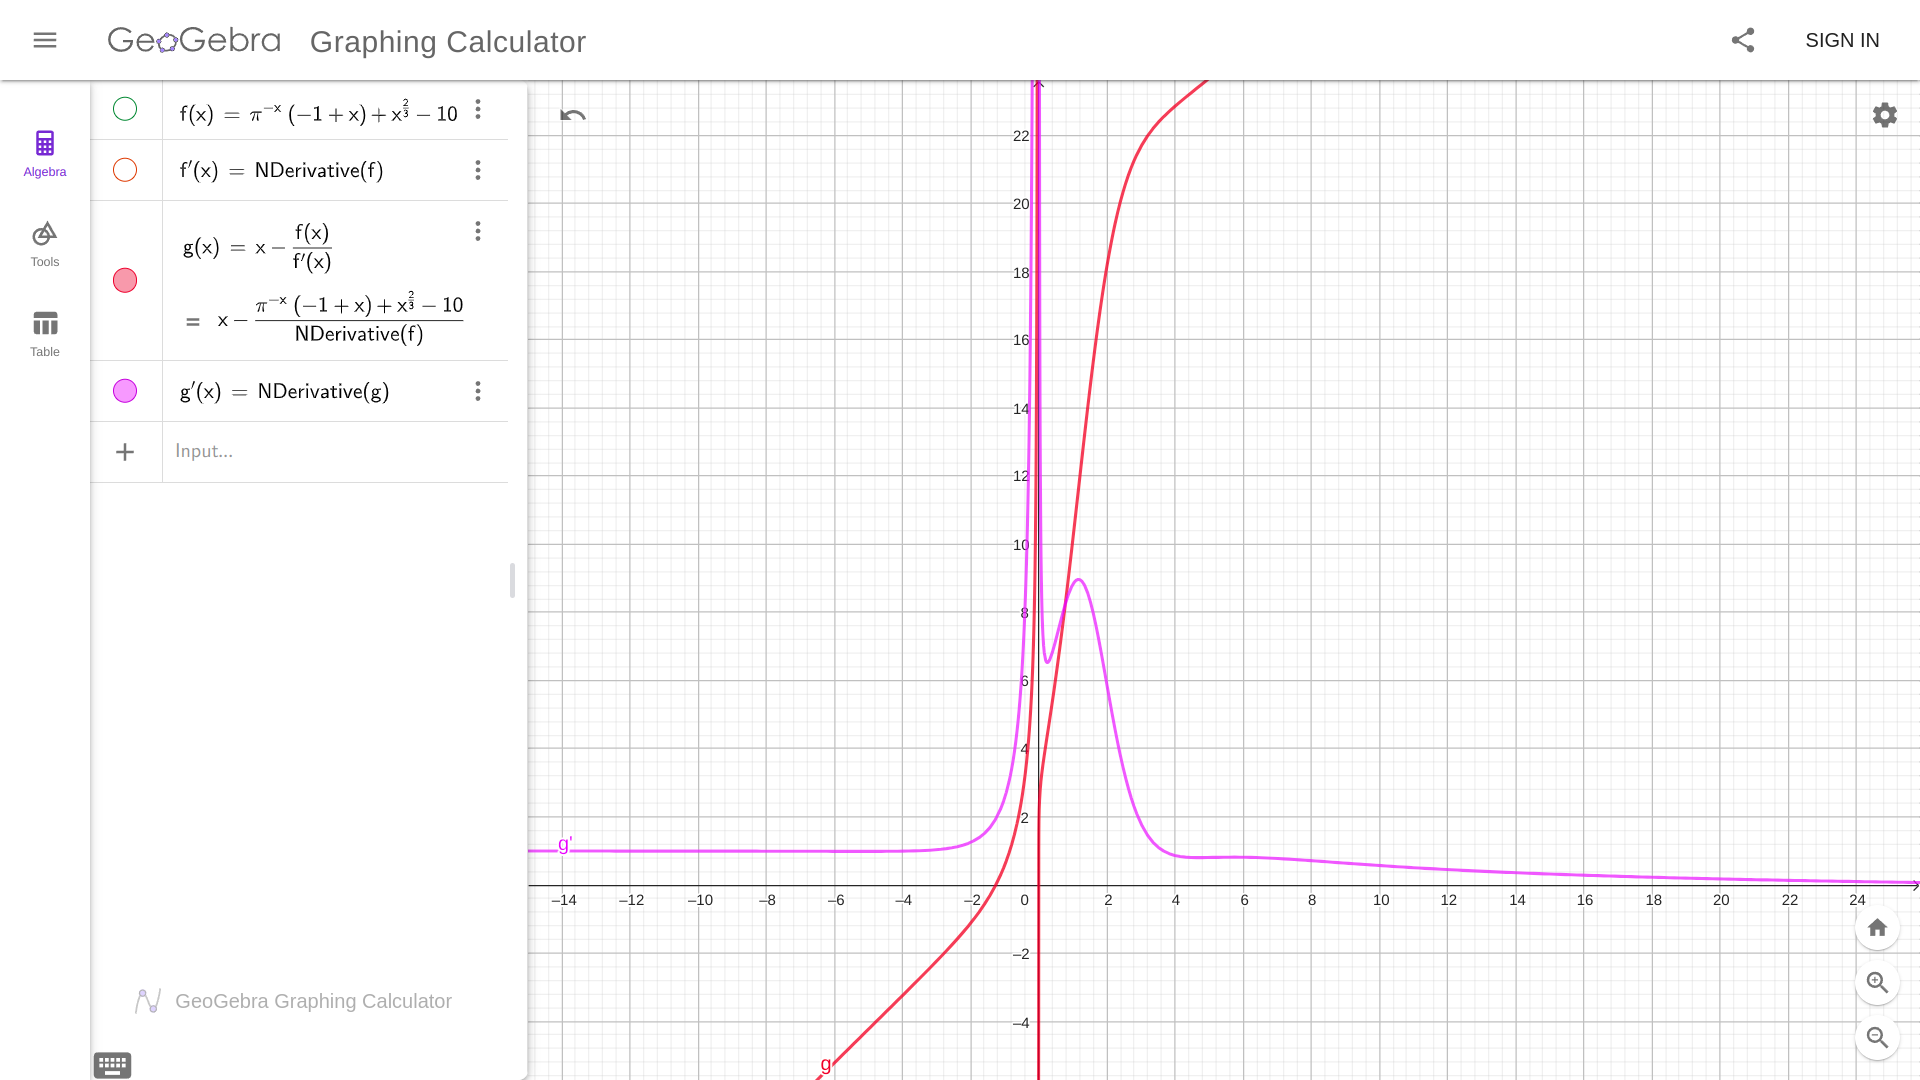
\includegraphics[width=\textwidth]{Figures/0. General/6.2.png}
        \caption{g(x) y g'(x)}
        \label{fig: g(x)}
    \end{subfigure}
\end{figure}

\subsection{1 pt}

Uno de los Skrull piensa buscar trabajo como modelo de Botero una vez se muden a
Medellín, pero necesita saber cuáles deben ser sus medidas de pecho $(x)$,
cintura $(y)$ y cadera $(z)$. Para esto, debe resolver el siguiente sistema de
ecuaciones por el método de Eliminación Gaussiana con pivoteo total
(dónde $C$ es los últimos dos dígitos de su cédula, que en este caso es el número 10):

\[
    \systeme*{9x - 6y + 6z = 100, 2x - y + 4z= 200, 7x - 8y + c= 300}
\]

Entregue el error en norma infinita y dé una respuesta a el Skrull sobre sus
medidas. Nos acaban de informar que se murió Botero, entonces no hay camello
para el Skrull, igual hagan el procedimiento.


Dado el sistema de ecuaciones

\[
    \systeme*{
        9x - 6y + 6z = 100,
        2x - y + 4z = 200,
        7x - 8y + 10z = 300
    }
\]

Tras aplicar el pivoteo total, reorganizamos las ecuaciones e incógnitas para tener el coeficiente con el mayor valor absoluto como pivote:

\[
    \systeme*{
        10z - 8y + 7x = 300,
        4z - y + 2x = 200,
        6z - 6y + 9x = 100
    }
\]

A continuación, simplificamos la primera ecuación dividiéndola por 10:

\[
    \systeme*{
        z - 0.8y + 0.7x = 30,
        4z - y + 2x = 200,
        6z - 6y + 9x = 100
    }
\]

Utilizamos la primera ecuación para eliminar \(z\) de las ecuaciones 2 y 3:

\[
    \systeme*{
        z - 0.8y + 0.7x = 30,
        -3x + 0.2y = 80,
        3x - 5.2y = 20
    }
\]

Resolviendo el sistema, podemos expresar \(x\) en términos de \(y\):

\[
    x = \frac{20 + 5.2y}{3}
\]

Sustituimos \(x\) en la segunda ecuación y resolvemos para \(y\). Luego, sustituimos los valores de \(x\) y \(y\) en la primera ecuación para obtener \(z\).

Finalmente, le informaríamos al Skrull sus medidas basadas en las soluciones \(x\), \(y\), y \(z\). Sin embargo, lamentablemente, debido al fallecimiento de Botero, no habrá oportunidad para que el Skrull trabaje como modelo.
